\documentclass[b4paper]{article}
\usepackage{amsmath,amssymb,kotex,paralist,graphicx,mdframed}
\usepackage[margin=1in]{geometry}
\usepackage{multicol}
\setlength{\columnseprule}{0.4pt}

\usepackage[inline]{enumitem}
\setlist[enumerate,1]{label=(\arabic*)}

\usepackage{tabto,pifont}
%\TabPositions{0.1\textwidth,0.2\textwidth,0.3\textwidth,0.4\textwidth}
\newcommand\taba[5]{\par\noindent
\ding{172}\:{\ensuremath{#1}}
\tabto{0.1\textwidth}\ding{173}\:\:{\ensuremath{#2}}
\tabto{0.2\textwidth}\ding{174}\:\:{\ensuremath{#3}}
\tabto{0.3\textwidth}\ding{175}\:\:{\ensuremath{#4}}
\tabto{0.4\textwidth}\ding{176}\:\:{\ensuremath{#5}}}

\newcommand\tabb[5]{\par\bigskip\noindent
\ding{172}\:\:{\ensuremath{#1}}
\tabto{0.16\textwidth}\ding{173}\:\:{\ensuremath{#2}}
\tabto{0.33\textwidth}\ding{174}\:\:{\ensuremath{#3}}\medskip\par\noindent
\ding{175}\:\:{\ensuremath{#4}}
\tabto{0.16\textwidth}\ding{176}\:\:{\ensuremath{#5}}}

\newcommand\tabc[5]{\par\bigskip\noindent
\ding{172}\:\:{\ensuremath{#1}}
\tabto{0.25\textwidth}\ding{173}\:\:{\ensuremath{#2}}\medskip\par\noindent
\ding{174}\:\:{\ensuremath{#3}}
\tabto{0.25\textwidth}\ding{175}\:\:{\ensuremath{#4}}\medskip\par\noindent
\ding{176}\:\:{\ensuremath{#5}}}

\newcommand\tabd[5]{\par\bigskip\noindent
\ding{172}\:{#1}\medskip\par\noindent
\ding{173}\:\:{#2}\medskip\par\noindent
\ding{174}\:\:{#3}\medskip\par\noindent
\ding{175}\:\:{#4}\medskip\par\noindent
\ding{176}\:\:{#5}}

%
\newcommand\one{\ding{172}}
\newcommand\two{\ding{173}}
\newcommand\three{\ding{174}}
\newcommand\four{\ding{175}}
\newcommand\five{\ding{176}}
%%% Counters
\newcounter{num}
%\newcounter{answer}

%%% Commands
\newcommand\prob
{\par\vspace{40pt}\noindent\refstepcounter{num} \textbf{문제 \thenum) }}
\newcommand\ans[1]
{\begin{flushright}답 : #1\end{flushright}}

%\let\emph\textsf
\renewcommand{\baselinestretch}{1.6}

\makeatletter
\newcommand{\newparallel}{\mathrel{\mathpalette\new@parallel\relax}}
\newcommand{\new@parallel}[2]{%
  \begingroup
  \sbox\z@{$#1T$}% get the height of an uppercase letter
  \resizebox{!}{\ht\z@}{\raisebox{\depth}{$\m@th#1/\mkern-5mu/$}}%
  \endgroup
}
\makeatother


\begin{document}
\begin{flushright}
\quad중학교 \qquad학년 \qquad반\qquad\qquad
이름 : \phantom{김선중}
\end{flushright}

\bigskip
\begin{multicols}{2}

%
\prob
두 수 48, 60의 최대공약수를 구하여라.
\taba369{12}{15}

%
\prob
세 수 6, 15, 27의 최소공배수를 구하여라.
\taba{108}{180}{215}{270}{540}

%
\prob
135의 약수의 개수를 구하여라.
\taba468{12}{16}

%
\prob
120의 약수의 개수를 구하여라.
\taba468{12}{16}

%
\prob
다음 중 가장 큰 수와 가장 작은 수의 합을 구하여라.
\begin{mdframed}
\[
\left(-\frac23\right)^2,
\quad
-\left(\frac23\right)^2,
\quad
-\frac{2^3}3,
\quad
\frac2{(-3)^3},
\quad
\frac{(-2)^2}3
\]
\end{mdframed}
\taba{-\frac43}{-\frac23}{0}{\frac23}{\frac43}

%
\prob
등식 \(ax-1=6(x-1)-3b\)가 \(x\)에 대한 항등식일 때, \(ab\)의 값을 구하면?
\taba{-10}{-5}05{10}

%
\prob
다음 일차방정식 \(7x+3=0\)을 풀어라.
\taba{-\frac73}{-\frac37}0{\frac37}{\frac73}

%
\prob
다음 일차방정식 \(\frac{x+2}4=1+\frac{x-1}3\)를 풀어라.
\taba{-2}{1}{4}{7}{10}
\vfill\null\columnbreak

%
\prob{}
유진이는 A에서 B까지 500m의 거리를 5m/s의 속력으로 뛰다가 B에서 C까지의 300m의 거리를 2m/s로 걸었다.
유진이가 A에서 C까지 이동할 때의 평균 속력을 구하여라.
\taba{2.8\text{m/s}}{3.2\text{m/s}}{3.6\text{m/s}}{4\text{m/s}}{4.4\text{m/s}}

%
\prob
집에서 서점까지 가는데 60km/h의 자동차로 가면 10km/h의 자전거로 가는 것보다 50분 빨리 도착한다고 한다. 그렇다면 40km/h의 오토바이로 가면 집에서 서점까지 몇 분 걸리겠는가?
\taba{10분}{12분}{15분}{20분}{30분}

%
\prob
세 점 \(O(0,0)\), \(P(0,4)\), \(Q(8,0)\)을 꼭짓점으로 하는 삼각형 \(OPQ\)의 넓이를 이등분하면서 원점을 지나는 직선을 나타내는 식은?
\tabb{y=\frac52x}{y=2x}{y=\frac32x}{y=\frac12x}{y=x}

%
\prob
아래 그래프는 지우와 민수가 200m 달리기를 할 때, 시간에 따른 출발점으로부터의 거리 변화를 나타내는 그래프이다.
다음 중 옳은 것은?
\begin{center}
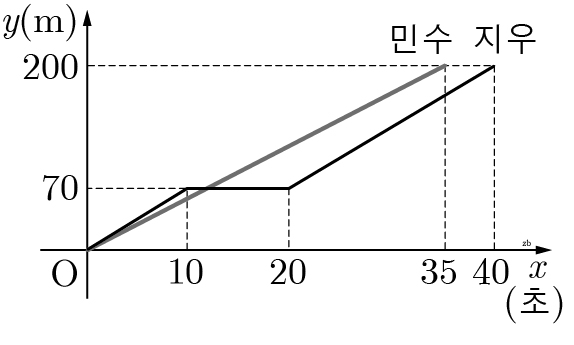
\includegraphics[width=.3\textwidth]{graph1}
\end{center}
\begin{mdframed}
\begin{enumerate}
\item[ㄱ.]
70m 지점에 지우가 민수보다 먼저 도착하였다.
\item[ㄴ.]
지우는 70m 지점에서 20초간 멈춰있었다.
\item[ㄷ.]
민수와 지우는 출발 후 도착 전까지 만나지 못했다.
\item[ㄹ.]
결승선에 먼저 도착한 사람은 민수이다.
\end{enumerate}
\end{mdframed}
\taba{\text{ㄱ, ㄴ}}{\text{ㄱ, ㄹ}}{\text{ㄴ, ㄷ}}{\text{ㄴ, ㄹ}}{\text{ㄷ, ㄹ}}

\newpage
%
\prob
수도꼭지를 틀어 계속 같은 양의 물이 흘러나오도록 한 후 다음 그림과 같은 모양의 병에 물을 받을 때, 병에 물을 받기 시작한 지 \(x\)초 후의 병에 물에 담긴 높이를 \(y\)cm라 하자.
이때, \(x\)와 \(y\) 사이의 관계를 나타낸 그래프는 다음 중 어떤 모양으로 나타나는가?
\begin{center}
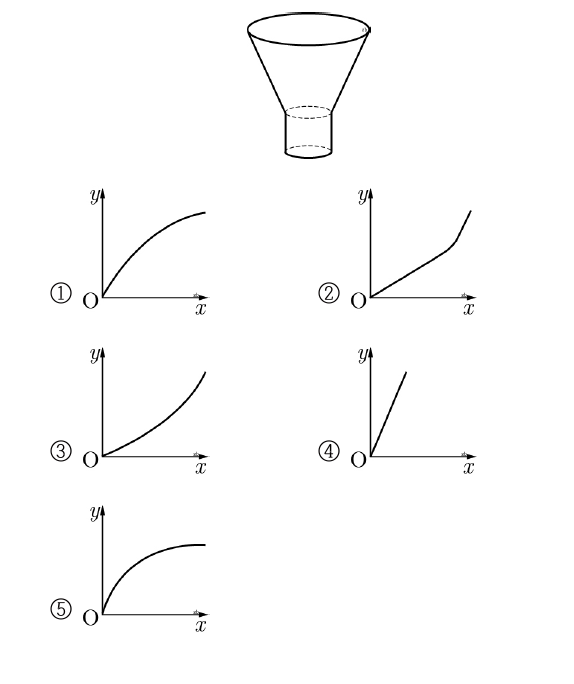
\includegraphics[width=.4\textwidth]{graph2}
\end{center}

%
\prob
다음 그림과 같이 반원 위에 있는 5개의 점 \(A\), \(B\), \(C\), \(D\), \(E\) 중에서 2개의 점으로 결정되는 선분의 개수를 \(a\), 직선의 개수를 \(b\)라고 할 때, \(a+b\)의 값을 구하면?
\begin{center}
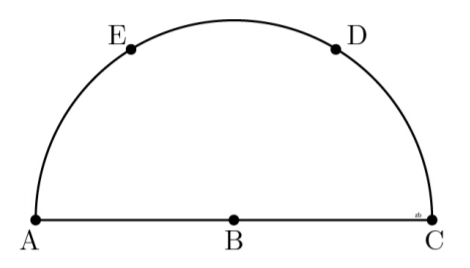
\includegraphics[width=.2\textwidth]{polygon1}
\end{center}
\taba{10}{14}{18}{22}{26}

%
\prob
다음 그림에서 \(l\newparallel m\)일 때, \(\angle x+\angle y\)의 값은?
\begin{center}
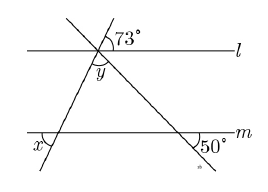
\includegraphics[width=.2\textwidth]{angle1}
\end{center}
\taba{110^\circ}{120^\circ}{130^\circ}{140^\circ}{150^\circ}
\vfill\null\columnbreak

%
\prob(주관식)
다음 그림에서 \(l\newparallel\)이고 사각형 \(ABCD\)가 정사각형일 때, \(\angle a\)와 \(\angle x\)의 크기를 각각 구하시오.
\begin{center}
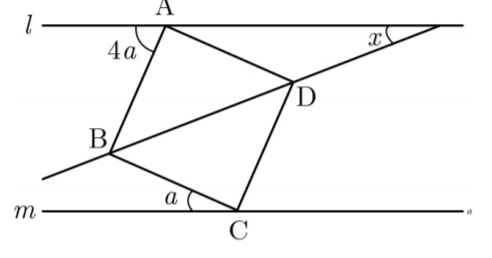
\includegraphics[width=.2\textwidth]{angle2}
\end{center}

%
\prob
다음 그림에서  \(\triangle ABC\)와 \(\triangle CDE\)는 정삼각형이다.
\(\triangle ACD\)와 합동인 삼각형과 이 때의 합동조건은?
\begin{center}
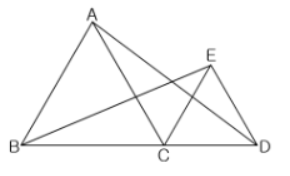
\includegraphics[width=.2\textwidth]{congruence1}
\end{center}
\tabc
{\triangle ABE, SSS합동}{\triangle BAE, SAS합동}
{\triangle BCE, SAS합동}{\triangle BCE, ASA합동}
{\triangle CBE, ASA합동}

%
\prob(주관식)
다음 그림의 정사각형 \(ABCD\)에서\\ \(\angle EAF=45^\circ\), \(\angle AEF=70^\circ\)일 때, \(\angle AFD\)의 크기를 구하시오.
\begin{center}
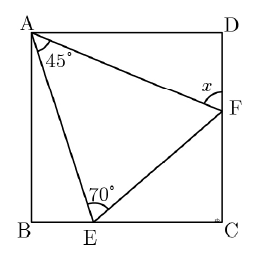
\includegraphics[width=.2\textwidth]{congruence2}
\end{center}

%
\prob
다음 그림에서 색칠한 부분의 둘레를 구하면?
\begin{center}
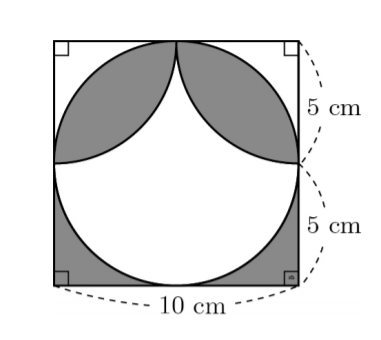
\includegraphics[width=.2\textwidth]{circumference}
\end{center}
\tabb
{10\pi\text{cm}}{(10\pi+20)\text{cm}}
{15\pi\text{cm}}{(15\pi+10)\text{cm}}
{(15\pi+20)\text{cm}}


\end{multicols}
\end{document}